\documentclass[11pt, a4paper]{article}
\usepackage[T1]{fontenc}
\usepackage[utf8]{inputenc}
\usepackage{fourier}
\usepackage{tgheros}
%\usepackage{sourcesanspro}
%\def\sfdefault{SourceSansPro-TLF}
\usepackage[cmex10]{amsmath}
\usepackage{amssymb}
\usepackage[pdftex]{graphicx}
\usepackage{epstopdf}
\epstopdfsetup{update}
\usepackage{fancyhdr}
\usepackage[twoside, margin=2.5cm, bindingoffset=0.0cm]{geometry}
\usepackage[numbers,sort&compress]{natbib}
\usepackage{url}
\usepackage{siunitx}
\sisetup{detect-all,input-product=*}%
\usepackage[labelformat=simple]{subcaption}
\captionsetup{font={footnotesize,sf},skip=2pt}
%\captionsetup[figure]{name=Fig.}
\captionsetup[sub]{labelfont={scriptsize},skip=0pt}
\renewcommand\thesubfigure{(\alph{subfigure})}
\usepackage[sectcntreset]{bibtopic}
\usepackage[compress,capitalize]{cleveref}
\usepackage{blindtext} % used to insert random text
%\usepackage{nicefrac}
\usepackage{microtype}

%\DeclareGraphicsRule{.wmf}{bmp}{}{}% declare WMF filename extension
\graphicspath{{Figures/}}

\newcommand{\super}[1]{\ensuremath{^{\mathrm{#1}}}}
\newcommand{\sub}[1]{\ensuremath{_{\mathrm{#1}}}}
\newcommand{\nicefrac}[2]{#1\big/#2}

\newcommand{\B}{ballistic}
\newcommand{\QB}{quasi-ballistic}
\newcommand{\DD}{drift-diffusion}
\newcommand{\sinv}{strong-inversion}
\newcommand{\winv}{weak-inversion}
\newcommand{\ns}{nanoscale}

\newcommand{\mosfet}{\textsc{{mosfet}}}
\newcommand{\qb}{quasi-ballistic}
\newcommand{\bal}{ballistic}
\newcommand{\Tsi}{\ensuremath{T\sub{si}}}
\newcommand{\Tox}{\ensuremath{T\sub{ox}}}
\newcommand{\Vg}{\ensuremath{V\sub{G}}}
\newcommand{\Vd}{\ensuremath{V\sub{D}}}
\newcommand{\Vs}{\ensuremath{V\sub{S}}}
\newcommand{\Vgdash}{\ensuremath{\Vg\super{'}}}
\newcommand{\phims} {\ensuremath{V\sub{fb}}}%{\phi\sub{ms}}
\newcommand{\psis}{\ensuremath{\psi\sub{s}}}
\newcommand{\psic}{\ensuremath{\psi\sub{c}}}
\newcommand{\psix}{\ensuremath{\psi(x)}}
\newcommand{\psiy}{\ensuremath{\psi(y)}}
\newcommand{\eox}{\ensuremath{\varepsilon\sub{ox}}}
\newcommand{\esi}{\ensuremath{\varepsilon\sub{si}}}
\newcommand{\Nd}{\ensuremath{N\sub{D}}}
\newcommand{\LGoverLc}{\nicefrac{L\sub{G}}{L\sub{c}}}
\newcommand{\lgate}{\textit{\textcolor{red}{long-gate}}}
\newcommand{\lgatesmall}{\textit{\textcolor{red!50}{long-gate}}}
\newcommand{\sgate}{\textit{\textcolor{darkblue}{short-gate}}}

%\newcommand{\figref}[1]{Fig.~\ref{#1}}

\newcolumntype{L}{>{$}l<{$}}
\newenvironment{Cases}{\begin{array}\{{lL}.}{\end{array}}

\setcounter{secnumdepth}{2}%
%\setcounter{tocdepth}{3}

\fancypagestyle{firstpage}{
\setlength{\headheight}{74pt}
\fancyhead[R]{
\includegraphics[width=0.25\textwidth]{epfl_logo}}
\fancyhead[L]{
\includegraphics[width=0.35\textwidth]{logo_uzh}}
%\fancyhead[L]{{\Large\textsc{\sffamily doctoral program in\\ microsystems \&
%microelectronics}}}%{DOCTORAL PROGRAM IN\\
% MICROSYSTEMS \& MICROELECTRONICS}}}
\fancyfoot{}}

\setlength{\parindent}{0pt}
\setlength{\parskip}{2ex plus 1ex minus 1ex}

\begin{document}
\vspace{150pt}
\title{\normalsize\bfseries Master Thesis (2016)\\
\vspace{20pt}
\Large\bfseries AFM Developement and Antibiotics Resistance Detection
% * <massimiliano.bertacchi@uzh.ch> 2016-07-09T12:22:04.899Z:
%
% > * <massimiliano.bertacchi@uzh.ch>
%
% Inserire Mail Sotto piede
%
% ^.
% * <massimiliano.bertacchi@uzh.ch> 2016-07-09T12:18:51.655Z:
%
% > Large\bfseries AFM Developement and Antibiotics Resistance Detection
%
% Fare diventare più grande
%
% ^.
%\vspace{10pt}
%\textit{Intermediate Report}}
}

\author{Massimiliano Bertacchi}
% * <massimiliano.bertacchi@uzh.ch> 2016-07-09T14:17:18.415Z:
%
% ^.
% * <massimiliano.bertacchi@uzh.ch> 2016-07-09T14:17:11.567Z:
%
% Completare Informazioni dal Testo di riferimento di Zurigo
%
% ^.
\maketitle %

\thispagestyle{firstpage}
\vspace{4cm}
\begin{tabular}{m{6cm} m{5cm} m{3cm}}
                 %\hline
                 % after \\: \hline or \cline{col1-col2} \cline{col3-col4} ...
                 \bfseries{Report Type:} & Intermediate & \\\\\\
                 \bfseries{Master Student:} & Massimiliano Bertacchi & \dotfill{} \\\\\\
                 \bfseries{Matricl n°:} & 414 12 212 ... & \dotfill{} \\\\\\
% * <massimiliano.bertacchi@uzh.ch> 2016-07-09T12:19:17.983Z:
%
% Mettere il vero numero di matricola (e guardare come si scrive in inglese)
%
% ^.
                 \bfseries{Thesis Director:} & Dr. S. Kasas & \dotfill{} \\\\\\
                 \bfseries{Date:} & \today & \\\\\\
 %               \hline
               \end{tabular}%
\newpage
\pagestyle{fancy}
\fancyhead{} % Clear all header fields
\setlength{\headheight}{24pt}
%\fancyhead[LE,RO]{\thepage} %
\fancyhead[CE,CO]{{Master Thesis (2016)}} %
\setlength{\headheight}{74pt}
\begin{tabular}{m{8cm} m{5cm} m{4cm}}
		 \bfseries{} & Ciò che rende bello il deserto é che, da qualche parte, nasconde un pozzo... \\
         \bfseries{} A. St. Exupery
% * <massimiliano.bertacchi@uzh.ch> 2016-07-09T12:19:47.929Z:
%
% >  A. St. Exupery
%
% Spostare a destra e cambiare la citazione
%
% ^.
 \end{tabular}%
\fancyfoot{} % Clear all footer fields
\fancyfoot[RE,LO]{\thepage}

\newpage
\tableofcontents %qui dovrei mettere l'indice

\newpage
\setcounter{page}{1}
\pagestyle{fancy}
\fancyhead{} % Clear all header fields
\setlength{\headheight}{24pt}
%\fancyhead[LE,RO]{\thepage} %
\fancyhead[CE,CO]{{Master Thesis (2016)}} %
%\fancyfoot{} % Clear all footer fields
%\fancyfoot[RE,LO]{\thepage}
%\fancyfoot[RE,LO]{\textit{\copyright M.Bertacchi}} %
%\fancyfoot[LE,RO]{\textit{%\today}} %

\section{Introduction}
\blindtext

\section{Work Objectives}
\blindtext

The goals of this work are as following: 
\begin{itemize}
    \item Understanding the behavior of ballisticity in nanoscale \mosfet{}s focusing especially on
    the electrostatics.
    \item Modeling the charge
    and potential in \bal{} and \qb{} double-gate \mosfet{}{}s in a semi-empirical manner that is
    more approachable to a designer.
\end{itemize}

\section{Methods}
\subsection{NanoAFM Technology }
\Blindtext
\begin{figure}[t]
\centering
	\begin{subfigure}{0.245\linewidth}
		\centering
		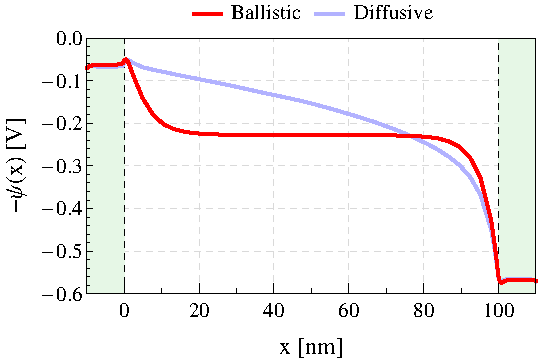
\includegraphics[width=1\linewidth]{potxBallDiff100}
		\caption{}\label{fig:1a}
	\end{subfigure}
	\begin{subfigure}{0.245\linewidth}
		\centering
		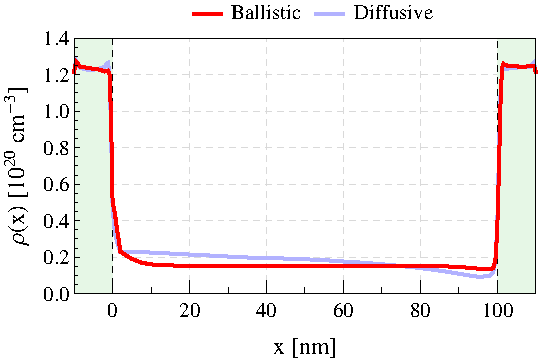
\includegraphics[width=1\linewidth]{ndxBallDiff100}
		\caption{}\label{fig:1b}
	\end{subfigure}
	\begin{subfigure}{0.245\linewidth}
		\centering
		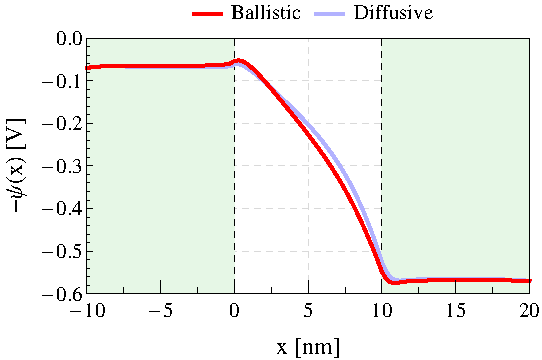
\includegraphics[width=1\linewidth]{potxBallDiff10}
		\caption{}\label{fig:1c}
	\end{subfigure}
	\begin{subfigure}{0.245\linewidth}
		\centering
		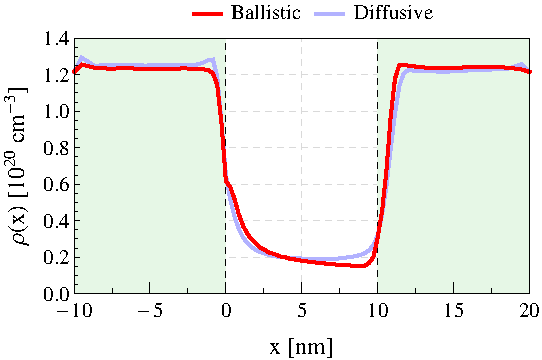
\includegraphics[width=1\linewidth]{ndxBallDiff10}
		\caption{}\label{fig:1d}
	\end{subfigure}
	\caption{\subref{fig:1a},\subref{fig:1c} Potential
	profile \subref{fig:1b},\subref{fig:1d} Carrier density
	profile of the \SIlist{10;100}{\nm} ballistic and diffusive devices.
	$\Vd=$\SI{0.5}{V}, $\Vs=$\SI{0}{V}.}
	\label{fig:1}
\end{figure}%

\subsection{Bacteria and Antibiotics}
\Blindtext

\begin{figure}[t]
    \centering 
    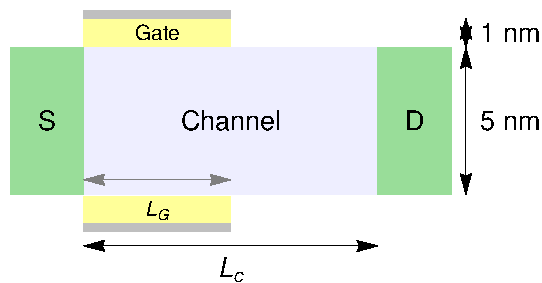
\includegraphics[width=0.25\columnwidth]{pgmos} \caption{Geometry of the proposed
    partially gated \textsc{dgsoi} \mosfet{}. %used for the Monte-Carlo
% simulations.
    The channel length $L\sub{c}$ is the length of the semiconductor between the source and drain
    junctions. The gate length $L\sub{G}$ is the length of the channel covered by the metal gate.
    This structure was simulated for $\LGoverLc=$ \numlist{0.1;0.3;0.5;0.9;1}.}
\label{fig:1:1}
\end{figure}%

\begin{figure}[b]
\centering
	\begin{subfigure}{0.245\linewidth}
		\centering
		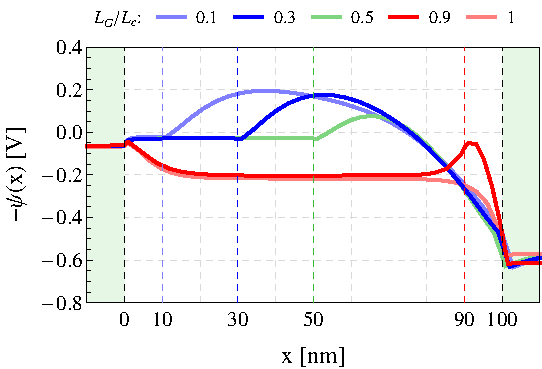
\includegraphics[width=1\linewidth]{potxPG100}
%		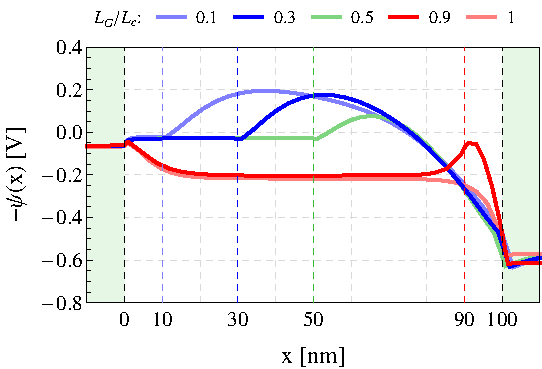
\includegraphics{potxPG100}
		\caption{}\label{fig:3:2a}
	\end{subfigure}
	\begin{subfigure}{0.245\linewidth}
		\centering
		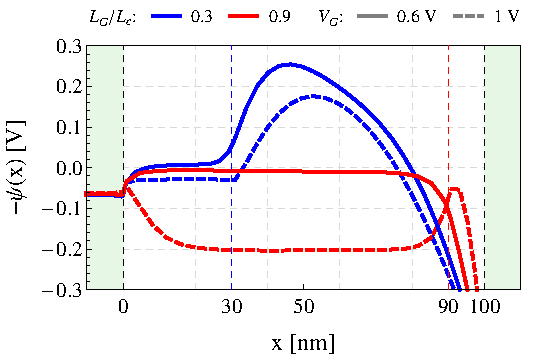
\includegraphics[width=1\linewidth]{potxPG100vg0610}
		\caption{}\label{fig:3:4a}
	\end{subfigure}
	\begin{subfigure}{0.245\linewidth}
		\centering
		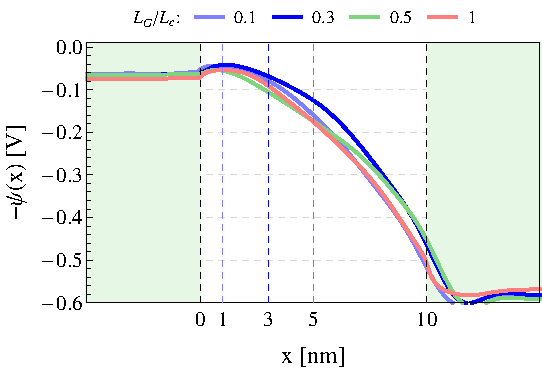
\includegraphics[width=1\linewidth]{potxPG10}
		\caption{}\label{fig:3:3a}
	\end{subfigure}
	\begin{subfigure}{0.245\linewidth}
		\centering
		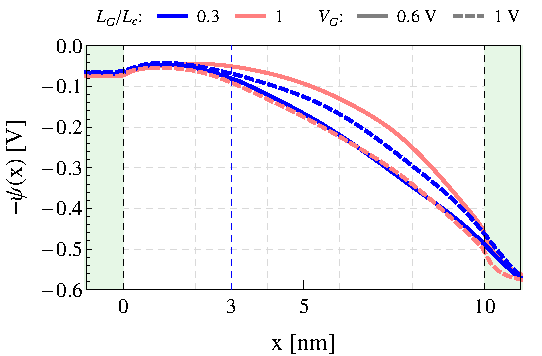
\includegraphics[width=1\linewidth]{potxPG10vg0610_new}
		\caption{}\label{fig:3:5a}
	\end{subfigure}
	\begin{subfigure}{0.245\linewidth}
		\centering
		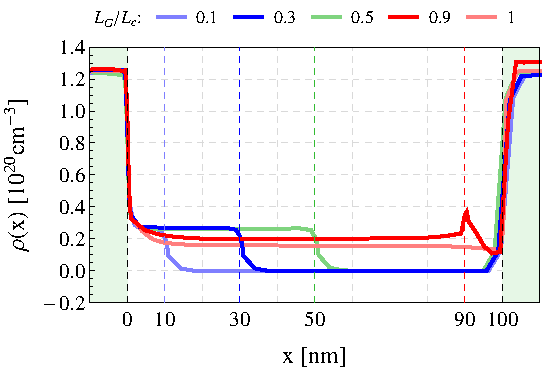
\includegraphics[width=1\linewidth]{ndxPG100}
%		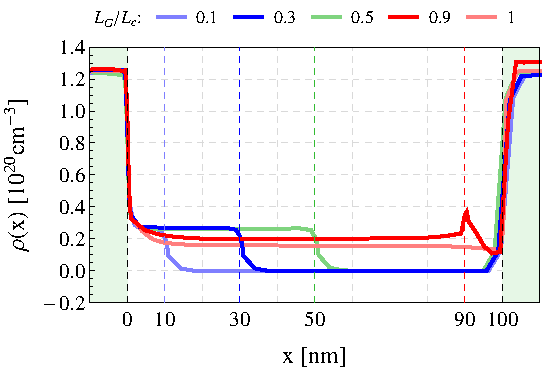
\includegraphics{ndxPG100}
		\caption{}\label{fig:3:2b}
	\end{subfigure}
	\begin{subfigure}{0.245\linewidth}
		\centering
		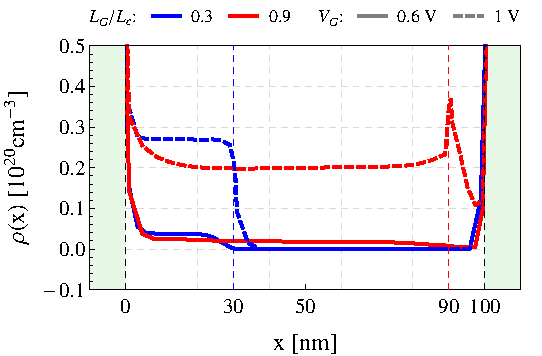
\includegraphics[width=1\linewidth]{ndxPG100vg0610}
		\caption{}\label{fig:3:4b}
	\end{subfigure}
	\begin{subfigure}{0.245\linewidth}
		\centering
		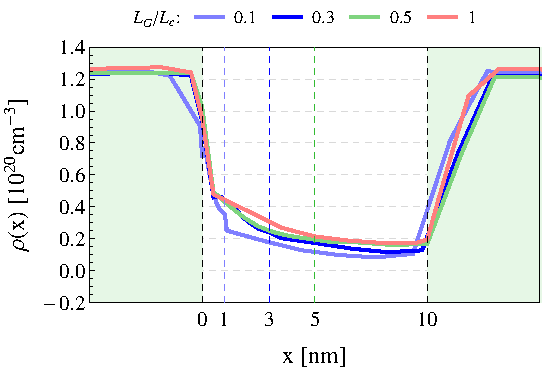
\includegraphics[width=1\linewidth]{ndxPG10}
		\caption{}\label{fig:3:3b}
	\end{subfigure}
	\begin{subfigure}{0.245\linewidth}
		\centering
		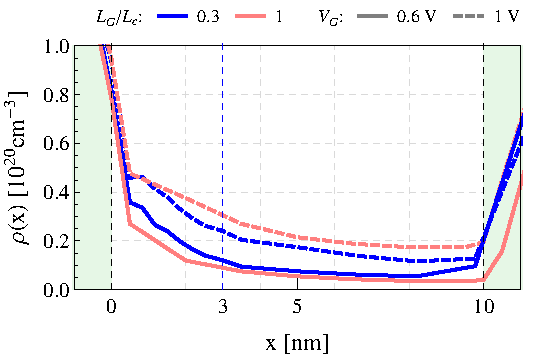
\includegraphics[width=1\linewidth]{ndxPG10vg0610_new}
		\caption{}\label{fig:3:5b}
	\end{subfigure}
	\caption{\subref{fig:3:2a},\subref{fig:3:4a},\subref{fig:3:3a},\subref{fig:3:5a} Potential
	profile \subref{fig:3:2b},\subref{fig:3:4b},\subref{fig:3:3b},\subref{fig:3:5b} Carrier density
	profile of the \SIlist{10;100}{\nm} partial-gate devices with different
	\nicefrac{L\sub{G}}{L\sub{c}} ratios.
	$\Vd=$\SI{0.5}{V}, $\Vs=$\SI{0}{V}}
	\label{fig:3:2}
\end{figure}%
    
\subsection{Data Analysis}
\blindtext

\subsection{Subsection heading 3}
\blindtext

\blindtext

\section{Personal Work}
Writing and editing of the PhD dissertation has begun and is expected to be finished by the end of
June 2014.

\section{Results}
\subsection{}

\section{Current State of the Work}
Writing and editing of the PhD dissertation has begun and is expected to be finished by the end of
June 2014.



\section{Calendar of Upcoming Work}
\begin{tabular}{p{0.5\textwidth}  l}
%\toprule
  Submission of the thesis & June 2014\\\\
  Private thesis defense & August 2014
%\bottomrule  
\end{tabular}%

\newpage
\bibliographystyle{IEEEtranN}
\begin{btSect}[IEEEtranN]{AnnualReport2014}
\section{Scientific Publications, Presentations, Conferences}
\btPrintAll
\end{btSect}

\begin{btSect}[IEEEtran]{BallisticVirtualSource}
\section{References}
%\btPrintCited
\btPrintAll
\end{btSect}

\end{document}